%%%%%%%%%%%%%%%%%%%%%%%%%%%%%%%%%%%%%%%%%
%  My documentation report
%  Objective: Explain what I did and how, so someone can continue with the investigation
%
% Important note:
% Chapter heading images should have a 2:1 width:height ratio,
% e.g. 920px width and 460px height.
%
%%%%%%%%%%%%%%%%%%%%%%%%%%%%%%%%%%%%%%%%%

%----------------------------------------------------------------------------------------
%	PACKAGES AND OTHER DOCUMENT CONFIGURATIONS
%----------------------------------------------------------------------------------------

\documentclass[11pt,fleqn]{book} % Default font size and left-justified equations

\usepackage[top=3cm,bottom=3cm,left=3.2cm,right=3.2cm,headsep=10pt,letterpaper]{geometry} % Page margins

\usepackage{xcolor} % Required for specifying colors by name
\definecolor{ocre}{RGB}{52,177,201} % Define the orange color used for highlighting throughout the book

% Font Settings
\usepackage{avant} % Use the Avantgarde font for headings
%\usepackage{times} % Use the Times font for headings
\usepackage{mathptmx} % Use the Adobe Times Roman as the default text font together with math symbols from the Sym­bol, Chancery and Com­puter Modern fonts

\usepackage{microtype} % Slightly tweak font spacing for aesthetics
\usepackage[utf8]{inputenc} % Required for including letters with accents
\usepackage[T1]{fontenc} % Use 8-bit encoding that has 256 glyphs

% Bibliography
\usepackage[style=alphabetic,sorting=nyt,sortcites=true,autopunct=true,babel=hyphen,hyperref=true,abbreviate=false,backref=true,backend=biber]{biblatex}
\addbibresource{bibliography.bib} % BibTeX bibliography file
\defbibheading{bibempty}{}

%----------------------------------------------------------------------------------------
%	VARIOUS REQUIRED PACKAGES
%----------------------------------------------------------------------------------------

\usepackage{titlesec} % Allows customization of titles

\usepackage{graphicx} % Required for including pictures
\graphicspath{{Pictures/}} % Specifies the directory where pictures are stored

\usepackage{lipsum} % Inserts dummy text

\usepackage{tikz} % Required for drawing custom shapes

\usepackage[english]{babel} % English language/hyphenation

\usepackage{enumitem} % Customize lists
\setlist{nolistsep} % Reduce spacing between bullet points and numbered lists

\usepackage{booktabs} % Required for nicer horizontal rules in tables

\usepackage{eso-pic} % Required for specifying an image background in the title page

%----------------------------------------------------------------------------------------
%	MAIN TABLE OF CONTENTS
%----------------------------------------------------------------------------------------

\usepackage{titletoc} % Required for manipulating the table of contents

\contentsmargin{0cm} % Removes the default margin
% Chapter text styling
\titlecontents{chapter}[1.25cm] % Indentation
{\addvspace{15pt}\large\sffamily\bfseries} % Spacing and font options for chapters
{\color{ocre!60}\contentslabel[\Large\thecontentslabel]{1.25cm}\color{ocre}} % Chapter number
{}  
{\color{ocre!60}\normalsize\sffamily\bfseries\;\titlerule*[.5pc]{.}\;\thecontentspage} % Page number
% Section text styling
\titlecontents{section}[1.25cm] % Indentation
{\addvspace{5pt}\sffamily\bfseries} % Spacing and font options for sections
{\contentslabel[\thecontentslabel]{1.25cm}} % Section number
{}
{\sffamily\hfill\color{black}\thecontentspage} % Page number
[]
% Subsection text styling
\titlecontents{subsection}[1.25cm] % Indentation
{\addvspace{1pt}\sffamily\small} % Spacing and font options for subsections
{\contentslabel[\thecontentslabel]{1.25cm}} % Subsection number
{}
{\sffamily\;\titlerule*[.5pc]{.}\;\thecontentspage} % Page number
[] 

%----------------------------------------------------------------------------------------
%	MINI TABLE OF CONTENTS IN CHAPTER HEADS
%----------------------------------------------------------------------------------------

% Section text styling
\titlecontents{lsection}[0em] % Indendating
{\footnotesize\sffamily} % Font settings
{}
{}
{}

% Subsection text styling
\titlecontents{lsubsection}[.5em] % Indentation
{\normalfont\footnotesize\sffamily} % Font settings
{}
{}
{}
 
%----------------------------------------------------------------------------------------
%	PAGE HEADERS
%----------------------------------------------------------------------------------------

\usepackage{fancyhdr} % Required for header and footer configuration

\pagestyle{fancy}
\renewcommand{\chaptermark}[1]{\markboth{\sffamily\normalsize\bfseries\chaptername\ \thechapter.\ #1}{}} % Chapter text font settings
\renewcommand{\sectionmark}[1]{\markright{\sffamily\normalsize\thesection\hspace{5pt}#1}{}} % Section text font settings
\fancyhf{} \fancyhead[LE,RO]{\sffamily\normalsize\thepage} % Font setting for the page number in the header
\fancyhead[LO]{\rightmark} % Print the nearest section name on the left side of odd pages
\fancyhead[RE]{\leftmark} % Print the current chapter name on the right side of even pages
\renewcommand{\headrulewidth}{0.5pt} % Width of the rule under the header
\addtolength{\headheight}{2.5pt} % Increase the spacing around the header slightly
\renewcommand{\footrulewidth}{0pt} % Removes the rule in the footer
\fancypagestyle{plain}{\fancyhead{}\renewcommand{\headrulewidth}{0pt}} % Style for when a plain pagestyle is specified

% Removes the header from odd empty pages at the end of chapters
\makeatletter
\renewcommand{\cleardoublepage}{
\clearpage\ifodd\c@page\else
\hbox{}
\vspace*{\fill}
\thispagestyle{empty}
\newpage
\fi}

%----------------------------------------------------------------------------------------
%	THEOREM STYLES
%----------------------------------------------------------------------------------------

\usepackage{amsmath,amsfonts,amssymb,amsthm} % For math equations, theorems, symbols, etc

\newcommand{\intoo}[2]{\mathopen{]}#1\,;#2\mathclose{[}}
\newcommand{\ud}{\mathop{\mathrm{{}d}}\mathopen{}}
\newcommand{\intff}[2]{\mathopen{[}#1\,;#2\mathclose{]}}
\newtheorem{notation}{Notation}[chapter]

%%%%%%%%%%%%%%%%%%%%%%%%%%%%%%%%%%%%%%%%%%%%%%%%%%%%%%%%%%%%%%%%%%%%%%%%%%%
%%%%%%%%%%%%%%%%%%%% dedicated to boxed/framed environements %%%%%%%%%%%%%%
%%%%%%%%%%%%%%%%%%%%%%%%%%%%%%%%%%%%%%%%%%%%%%%%%%%%%%%%%%%%%%%%%%%%%%%%%%%
\newtheoremstyle{ocrenumbox}% % Theorem style name
{0pt}% Space above
{0pt}% Space below
{\normalfont}% % Body font
{}% Indent amount
{\small\bf\sffamily\color{ocre}}% % Theorem head font
{\;}% Punctuation after theorem head
{0.25em}% Space after theorem head
{\small\sffamily\color{ocre}\thmname{#1}\nobreakspace\thmnumber{\@ifnotempty{#1}{}\@upn{#2}}% Theorem text (e.g. Theorem 2.1)
\thmnote{\nobreakspace\the\thm@notefont\sffamily\bfseries\color{black}---\nobreakspace#3.}} % Optional theorem note
\renewcommand{\qedsymbol}{$\blacksquare$}% Optional qed square

\newtheoremstyle{blacknumex}% Theorem style name
{5pt}% Space above
{5pt}% Space below
{\normalfont}% Body font
{} % Indent amount
{\small\bf\sffamily}% Theorem head font
{\;}% Punctuation after theorem head
{0.25em}% Space after theorem head
{\small\sffamily{\tiny\ensuremath{\blacksquare}}\nobreakspace\thmname{#1}\nobreakspace\thmnumber{\@ifnotempty{#1}{}\@upn{#2}}% Theorem text (e.g. Theorem 2.1)
\thmnote{\nobreakspace\the\thm@notefont\sffamily\bfseries---\nobreakspace#3.}}% Optional theorem note

\newtheoremstyle{blacknumbox} % Theorem style name
{0pt}% Space above
{0pt}% Space below
{\normalfont}% Body font
{}% Indent amount
{\small\bf\sffamily}% Theorem head font
{\;}% Punctuation after theorem head
{0.25em}% Space after theorem head
{\small\sffamily\thmname{#1}\nobreakspace\thmnumber{\@ifnotempty{#1}{}\@upn{#2}}% Theorem text (e.g. Theorem 2.1)
\thmnote{\nobreakspace\the\thm@notefont\sffamily\bfseries---\nobreakspace#3.}}% Optional theorem note

%%%%%%%%%%%%%%%%%%%%%%%%%%%%%%%%%%%%%%%%%%%%%%%%%%%%%%%%%%%%%%%%%%%%%%%%%%%
%%%%%%%%%%%%% dedicated to non-boxed/non-framed environements %%%%%%%%%%%%%
%%%%%%%%%%%%%%%%%%%%%%%%%%%%%%%%%%%%%%%%%%%%%%%%%%%%%%%%%%%%%%%%%%%%%%%%%%%
\newtheoremstyle{ocrenum}% % Theorem style name
{5pt}% Space above
{5pt}% Space below
{\normalfont}% % Body font
{}% Indent amount
{\small\bf\sffamily\color{ocre}}% % Theorem head font
{\;}% Punctuation after theorem head
{0.25em}% Space after theorem head
{\small\sffamily\color{ocre}\thmname{#1}\nobreakspace\thmnumber{\@ifnotempty{#1}{}\@upn{#2}}% Theorem text (e.g. Theorem 2.1)
\thmnote{\nobreakspace\the\thm@notefont\sffamily\bfseries\color{black}---\nobreakspace#3.}} % Optional theorem note
\renewcommand{\qedsymbol}{$\blacksquare$}% Optional qed square
\makeatother

% Defines the theorem text style for each type of theorem to one of the three styles above
\newcounter{dummy} 
\numberwithin{dummy}{section}
\theoremstyle{ocrenumbox}
\newtheorem{theoremeT}[dummy]{Theorem}
\newtheorem{problem}{Problem}[chapter]
\newtheorem{exerciseT}{Exercise}[chapter]
\theoremstyle{blacknumex}
\newtheorem{exampleT}{Example}[chapter]
\theoremstyle{blacknumbox}
\newtheorem{vocabulary}{Vocabulary}[chapter]
\newtheorem{definitionT}{Definition}[section]
\newtheorem{corollaryT}[dummy]{Corollary}
\theoremstyle{ocrenum}
\newtheorem{proposition}[dummy]{Proposition}

%----------------------------------------------------------------------------------------
%	DEFINITION OF COLORED BOXES
%----------------------------------------------------------------------------------------

\RequirePackage[framemethod=default]{mdframed} % Required for creating the theorem, definition, exercise and corollary boxes

% Theorem box
\newmdenv[skipabove=7pt,
skipbelow=7pt,
backgroundcolor=black!5,
linecolor=ocre,
innerleftmargin=5pt,
innerrightmargin=5pt,
innertopmargin=5pt,
leftmargin=0cm,
rightmargin=0cm,
innerbottommargin=5pt]{tBox}

% Exercise box	  
\newmdenv[skipabove=7pt,
skipbelow=7pt,
rightline=false,
leftline=true,
topline=false,
bottomline=false,
backgroundcolor=ocre!10,
linecolor=ocre,
innerleftmargin=5pt,
innerrightmargin=5pt,
innertopmargin=5pt,
innerbottommargin=5pt,
leftmargin=0cm,
rightmargin=0cm,
linewidth=4pt]{eBox}	

% Definition box
\newmdenv[skipabove=7pt,
skipbelow=7pt,
rightline=false,
leftline=true,
topline=false,
bottomline=false,
linecolor=ocre,
innerleftmargin=5pt,
innerrightmargin=5pt,
innertopmargin=0pt,
leftmargin=0cm,
rightmargin=0cm,
linewidth=4pt,
innerbottommargin=0pt]{dBox}	

% Corollary box
\newmdenv[skipabove=7pt,
skipbelow=7pt,
rightline=false,
leftline=true,
topline=false,
bottomline=false,
linecolor=gray,
backgroundcolor=black!5,
innerleftmargin=5pt,
innerrightmargin=5pt,
innertopmargin=5pt,
leftmargin=0cm,
rightmargin=0cm,
linewidth=4pt,
innerbottommargin=5pt]{cBox}

% Creates an environment for each type of theorem and assigns it a theorem text style from the "Theorem Styles" section above and a colored box from above
\newenvironment{theorem}{\begin{tBox}\begin{theoremeT}}{\end{theoremeT}\end{tBox}}
\newenvironment{exercise}{\begin{eBox}\begin{exerciseT}}{\hfill{\color{ocre}\tiny\ensuremath{\blacksquare}}\end{exerciseT}\end{eBox}}				  
\newenvironment{definition}{\begin{dBox}\begin{definitionT}}{\end{definitionT}\end{dBox}}	
\newenvironment{example}{\begin{exampleT}}{\hfill{\tiny\ensuremath{\blacksquare}}\end{exampleT}}		
\newenvironment{corollary}{\begin{cBox}\begin{corollaryT}}{\end{corollaryT}\end{cBox}}	

%----------------------------------------------------------------------------------------
%	REMARK ENVIRONMENT
%----------------------------------------------------------------------------------------

\newenvironment{remark}{\par\vspace{10pt}\small % Vertical white space above the remark and smaller font size
\begin{list}{}{
\leftmargin=35pt % Indentation on the left
\rightmargin=25pt}\item\ignorespaces % Indentation on the right
\makebox[-2.5pt]{\begin{tikzpicture}[overlay]
\node[draw=ocre!60,line width=1pt,circle,fill=ocre!25,font=\sffamily\bfseries,inner sep=2pt,outer sep=0pt] at (-15pt,0pt){\textcolor{ocre}{R}};\end{tikzpicture}} % Orange R in a circle
\advance\baselineskip -1pt}{\end{list}\vskip5pt} % Tighter line spacing and white space after remark

%----------------------------------------------------------------------------------------
%	SECTION NUMBERING IN THE MARGIN
%----------------------------------------------------------------------------------------

\makeatletter
\renewcommand{\@seccntformat}[1]{\llap{\textcolor{ocre}{\csname the#1\endcsname}\hspace{1em}}}                    
\renewcommand{\section}{\@startsection{section}{1}{\z@}
{-4ex \@plus -1ex \@minus -.4ex}
{1ex \@plus.2ex }
{\normalfont\large\sffamily\bfseries}}
\renewcommand{\subsection}{\@startsection {subsection}{2}{\z@}
{-3ex \@plus -0.1ex \@minus -.4ex}
{0.5ex \@plus.2ex }
{\normalfont\sffamily\bfseries}}
\renewcommand{\subsubsection}{\@startsection {subsubsection}{3}{\z@}
{-2ex \@plus -0.1ex \@minus -.2ex}
{.2ex \@plus.2ex }
{\normalfont\small\sffamily\bfseries}}                        
\renewcommand\paragraph{\@startsection{paragraph}{4}{\z@}
{-2ex \@plus-.2ex \@minus .2ex}
{.1ex}
{\normalfont\small\sffamily\bfseries}}

%----------------------------------------------------------------------------------------
%	HYPERLINKS IN THE DOCUMENTS
%----------------------------------------------------------------------------------------

% For an unclear reason, the package should be loaded now and not later
\usepackage{hyperref}
\hypersetup{hidelinks,backref=true,pagebackref=true,hyperindex=true,colorlinks=false,breaklinks=true,urlcolor= ocre,bookmarks=true,bookmarksopen=false,pdftitle={Title},pdfauthor={Author}}

%----------------------------------------------------------------------------------------
%	CHAPTER HEADINGS
%----------------------------------------------------------------------------------------

% The set-up below should be (sadly) manually adapted to the overall margin page septup controlled by the geometry package loaded in the main.tex document. It is possible to implement below the dimensions used in the goemetry package (top,bottom,left,right)... TO BE DONE

\newcommand{\thechapterimage}{}
\newcommand{\chapterimage}[1]{\renewcommand{\thechapterimage}{#1}}

% Numbered chapters with mini tableofcontents
\def\thechapter{\arabic{chapter}}
\def\@makechapterhead#1{
\thispagestyle{empty}
{\centering \normalfont\sffamily
\ifnum \c@secnumdepth >\m@ne
\if@mainmatter
\startcontents
\begin{tikzpicture}[remember picture,overlay]
\node at (current page.north west)
{\begin{tikzpicture}[remember picture,overlay]
\node[anchor=north west,inner sep=0pt] at (0,0) {\includegraphics[width=\paperwidth]{\thechapterimage}};
%%%%%%%%%%%%%%%%%%%%%%%%%%%%%%%%%%%%%%%%%%%%%%%%%%%%%%%%%%%%%%%%%%%%%%%%%%%%%%%%%%%%%
% Commenting the 3 lines below removes the small contents box in the chapter heading
%\fill[color=ocre!10!white,opacity=.6] (1cm,0) rectangle (8cm,-7cm);
%\node[anchor=north west] at (1.1cm,.35cm) {\parbox[t][8cm][t]{6.5cm}{\huge\bfseries\flushleft \printcontents{l}{1}{\setcounter{tocdepth}{2}}}};
\draw[anchor=west] (5cm,-9cm) node [rounded corners=20pt,fill=ocre!10!white,text opacity=1,draw=ocre,draw opacity=1,line width=1.5pt,fill opacity=.6,inner sep=12pt]{\huge\sffamily\bfseries\textcolor{black}{\thechapter. #1\strut\makebox[22cm]{}}};
%%%%%%%%%%%%%%%%%%%%%%%%%%%%%%%%%%%%%%%%%%%%%%%%%%%%%%%%%%%%%%%%%%%%%%%%%%%%%%%%%%%%%
\end{tikzpicture}};
\end{tikzpicture}}
\par\vspace*{230\p@}
\fi
\fi}

% Unnumbered chapters without mini tableofcontents (could be added though) 
\def\@makeschapterhead#1{
\thispagestyle{empty}
{\centering \normalfont\sffamily
\ifnum \c@secnumdepth >\m@ne
\if@mainmatter
\begin{tikzpicture}[remember picture,overlay]
\node at (current page.north west)
{\begin{tikzpicture}[remember picture,overlay]
\node[anchor=north west,inner sep=0pt] at (0,0) {\includegraphics[width=\paperwidth]{\thechapterimage}};
\draw[anchor=west] (5cm,-9cm) node [rounded corners=20pt,fill=ocre!10!white,fill opacity=.6,inner sep=12pt,text opacity=1,draw=ocre,draw opacity=1,line width=1.5pt]{\huge\sffamily\bfseries\textcolor{black}{#1\strut\makebox[22cm]{}}};
\end{tikzpicture}};
\end{tikzpicture}}
\par\vspace*{230\p@}
\fi
\fi
}
\makeatother % Insert the commands.tex file which contains the majority of the structure behind the template

\begin{document}

%----------------------------------------------------------------------------------------
%	TITLE PAGE
%----------------------------------------------------------------------------------------

\begingroup
\thispagestyle{empty}
\AddToShipoutPicture*{\put(0,0){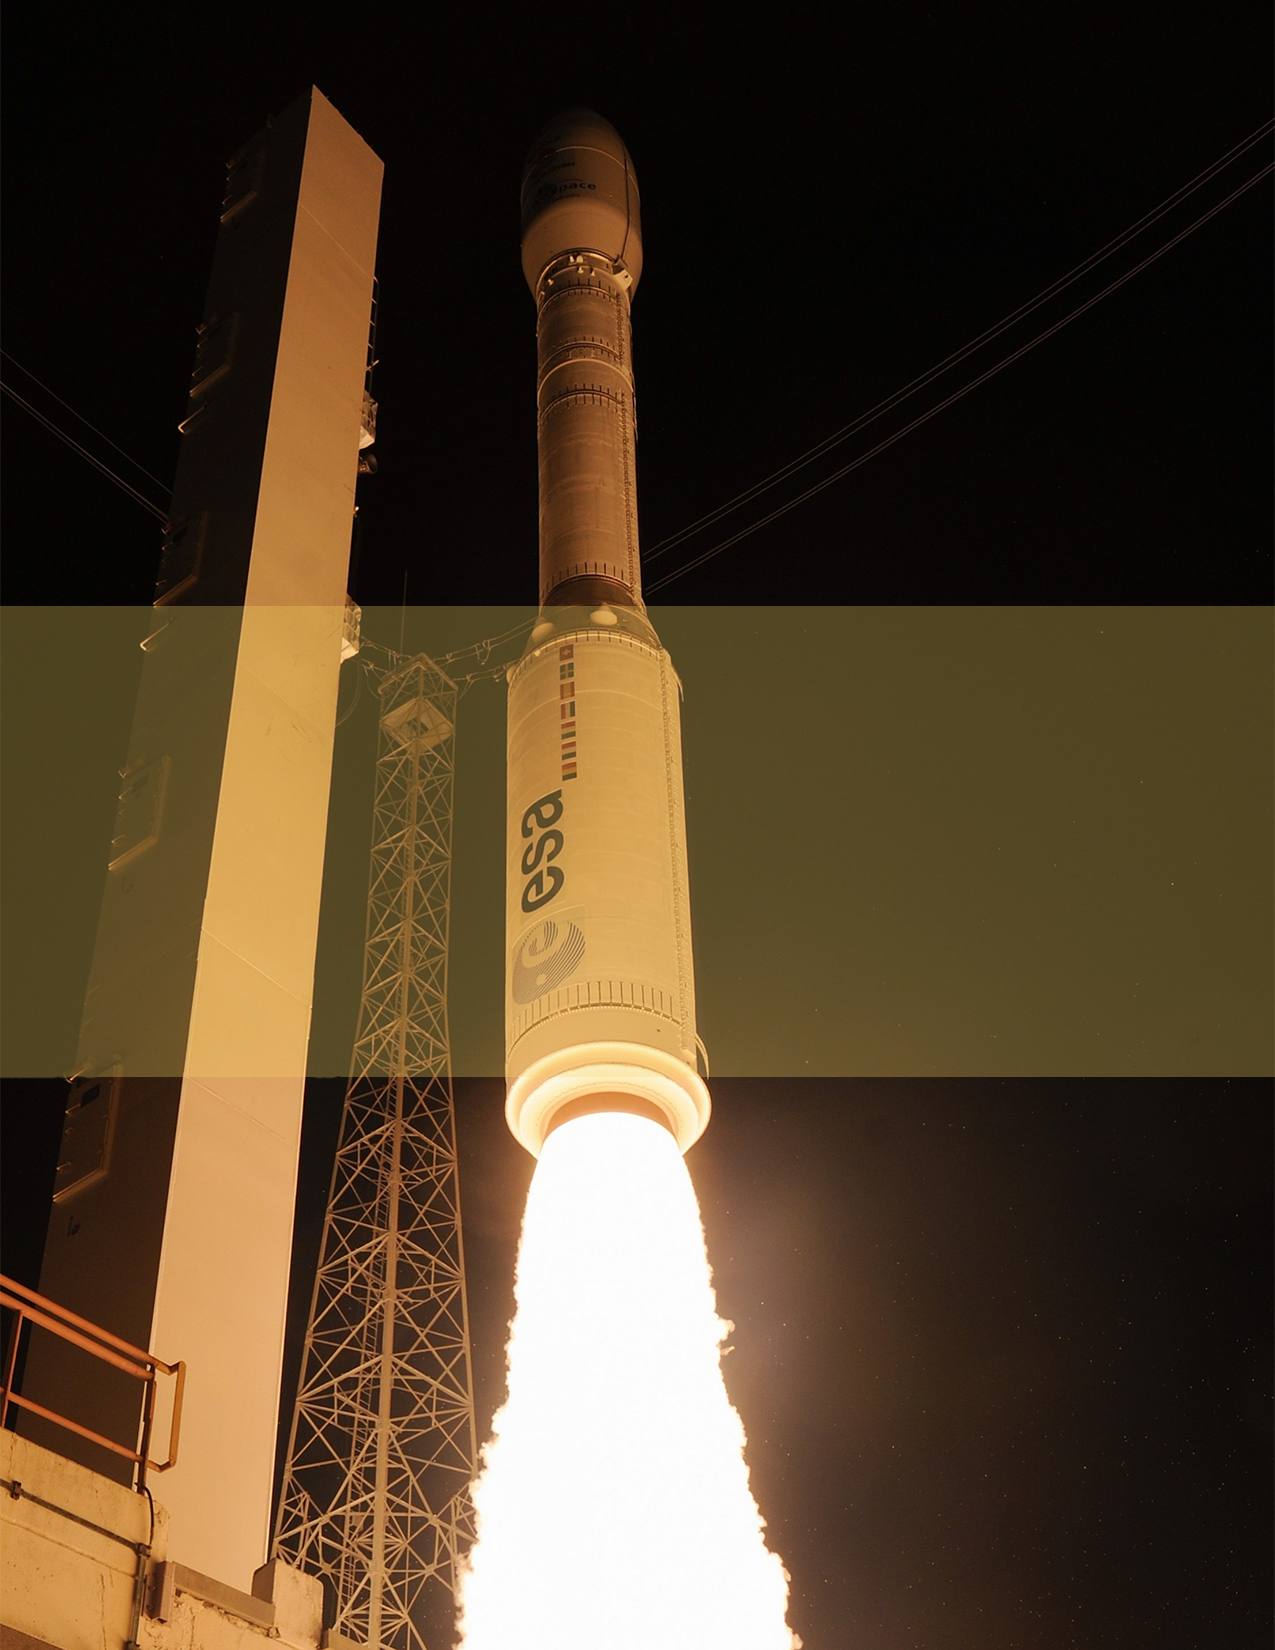
\includegraphics[scale=0.65]{Rocket}}} % Image background
\centering
\vspace*{8cm}
\par\normalfont\fontsize{35}{35}\sffamily\selectfont
\textbf{LISA Pathfinder}\\
{\LARGE European Space Agency}\par % Book title
\vspace*{1cm}
{\Huge Utkarsh Chauhan}\par % Author name
\endgroup
\let\cleardoublepage\clearpage
\chapterimage{new1.png} % Table of contents heading image

\pagestyle{empty} % No headers

\tableofcontents % Print the table of contents itself

\cleardoublepage % Forces the first chapter to start on an odd page so it's on the right

\pagestyle{fancy} % Print headers again

%----------------------------------------------------------------------------------------
%	CHAPTER 1
%----------------------------------------------------------------------------------------

\chapterimage{LISA_Pathfinder_in_low-Earth_orbit_C.png} % Chapter heading image

\chapter{Overview}

\section{Mission}\index{Motivation}
LISA Pathfinder is testing in flight the concept of low-frequency gravitational wave detection: it placed two test masses in a near-perfect gravitational free-fall, and is controlling and measuring their motion with unprecedented accuracy. To do this, it makes use of inertial sensors, a laser metrology system, a drag-free control system and an ultra-precise micro-propulsion system.

\section{Objective}\index{Objective}
The aim of the LISA Pathfinder mission is to demonstrate, in a space environment, that free-falling bodies follow geodesics – the equivalent of straight lines in a curved space – in spacetime, by more than two orders of magnitude better than any past, present or planned mission. Specifically, it must:
\begin{itemize}
\item Demonstrate drag-free and attitude control in a spacecraft with two free proof masses.
\item Test feasibility of laser interferometry with picometre resolution at low frequency, approaching 10-12 mHz-1/2 in the frequency band 1–30 mHz.
\item Test the endurance of the different instruments and hardware in the space environment.
\end{itemize}


\section{References}\index{Reference}
For more Information about LISA Pathfinder Visit:
		\begin{description}
        	\item[]\url{http://blogs.esa.int/}
            \item[]\url{http://spaceflight101.com/lisa-pathfinder/}
            \item[]\url{https://lisapathfinder.org/}
            \item[]\url{https://en.wikipedia.org/wiki/LISA_Pathfinder}
            \item[]\url{http://sci.esa.int/lisa-pathfinder/}
        \end{description}

\chapterimage{LaunchVehicle.png}

\chapter{Launch Vehicle and Ascent Mission}

\section{Vega Launch Vehicle}\index{First ideas}
Vega is a three-stage all-solid launch vehicle with an optional liquid fueled upper stage for re-start and precise injection capability. The launch vehicle stands 29.9 meters tall, has a main diameter of 3.03 meters and a liftoff mass of 137,000 Kilograms. The Rocket can lift up to 2,500 Kilograms of Payloads – depending on the target orbit.
\begin{figure}[h]
    \centering
    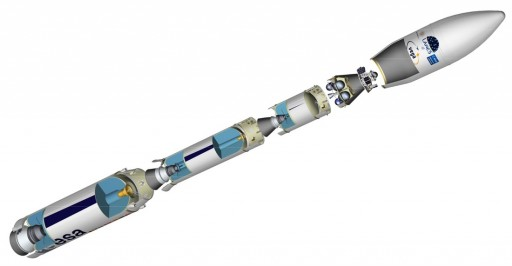
\includegraphics[width=1.0\textwidth]{5939181_orig-512x266.png}
    \caption{Disintegrated view of Vega - European Space Agency}
    \label{fig:awesome_image}
\end{figure}

\subsection{First Stage}
The P80FW first Stage of the Vega Vehicle burns for 106.8 seconds giving it an altitude of 50 Kilometers and a velocity of 1765 m/s . After which Stage 1 separates and Stage 2 ignites. 
\begin{figure}[h]
    \centering
    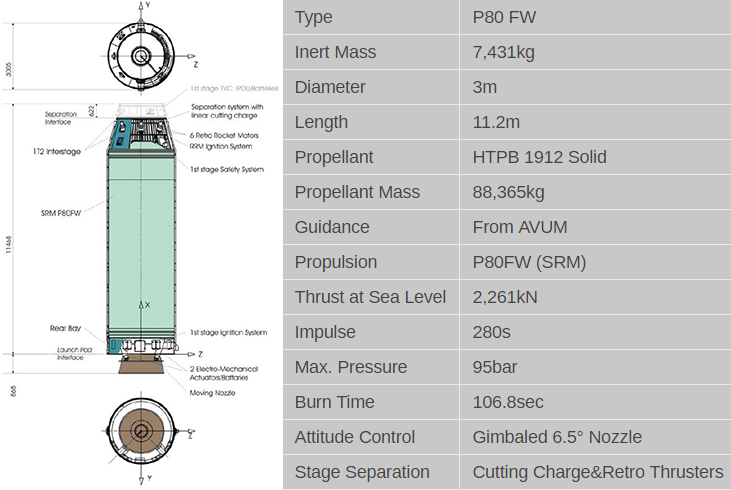
\includegraphics[width=0.9\textwidth]{Stage1.png}
    \caption{Vega First Stage Configuration and Data}
    \label{fig:super}
\end{figure}

\begin{figure}[h]
    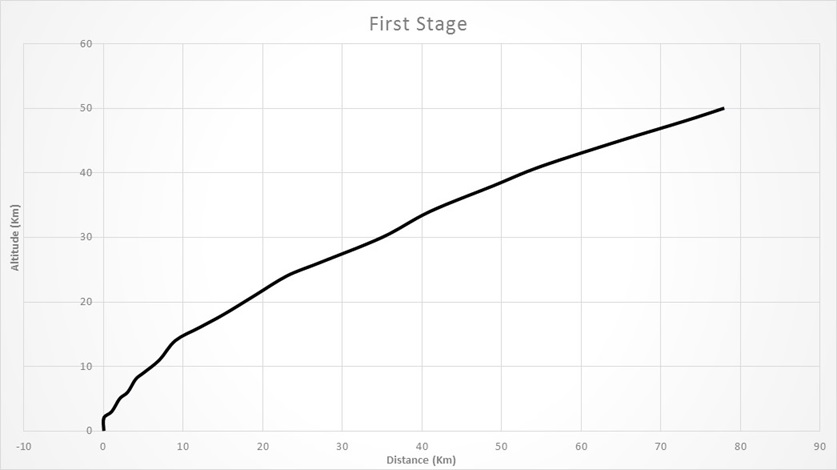
\includegraphics[width=0.56\textwidth]{Stage_1_Plot.jpg}
    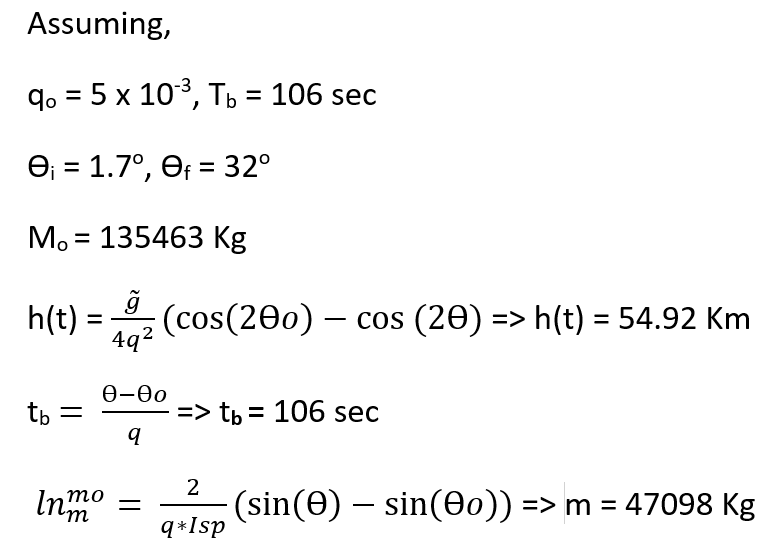
\includegraphics[width=0.44\textwidth]{Stage1_Cal.png}
    \caption{Stage 1 Trajectory Analysis}
    \label{fig:super}
\end{figure}

\newpage

\subsection{Second Stage}

The second stage ZEFIRO 23 Solid Rocket Motor burns for about 71.7 seconds giving the rocket a speed of 3847 m/s and reaching an altitude of 70.26 Kilometers after which it separates and 3rd stage ignites.  
\begin{figure}[h]
    \centering
    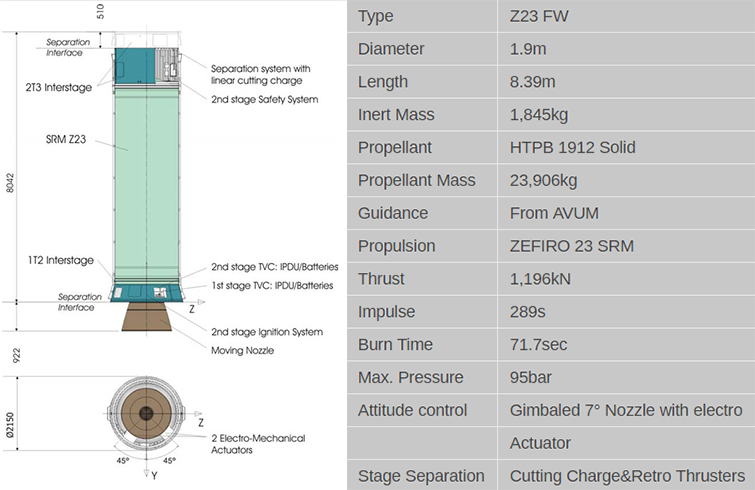
\includegraphics[width=0.95\textwidth]{Stage2.png}
    \caption{Vega Second Stage Configuration and Data}
    \label{fig:super}
\end{figure}

\begin{figure}[h]
    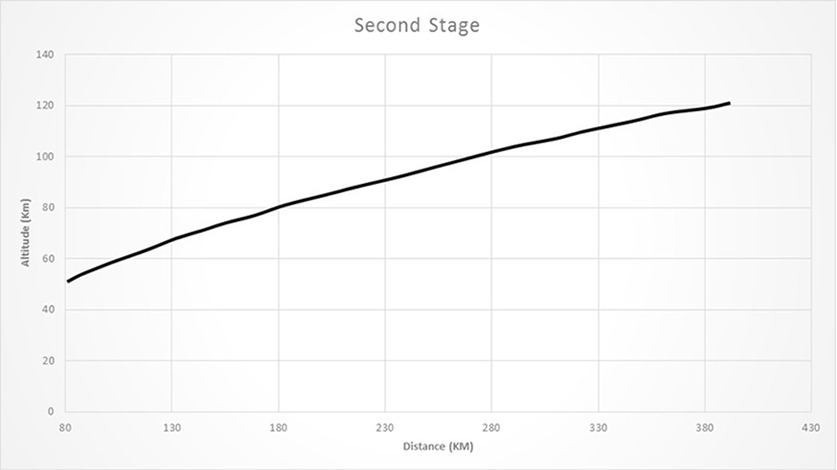
\includegraphics[width=0.56\textwidth]{Stage_2_Plot.jpg}
    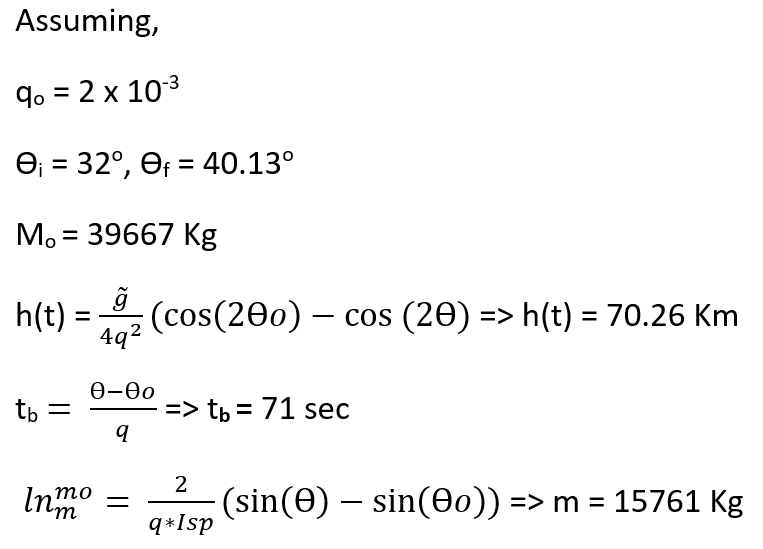
\includegraphics[width=0.44\textwidth]{Stage2_Cal.png}
    \caption{Stage 2 Trajectory Analysis}
    \label{fig:super}
\end{figure}
\clearpage
\subsection{Third Stage}

The ZEFIRO 9 solid motor burns for about 109.8 seconds giving vehicle an altitude of 193  Kilometers. During the Third Stage Payload Fairing separates at an altitude of 80.52 Kilometers.
\begin{figure}[h]
    \centering
    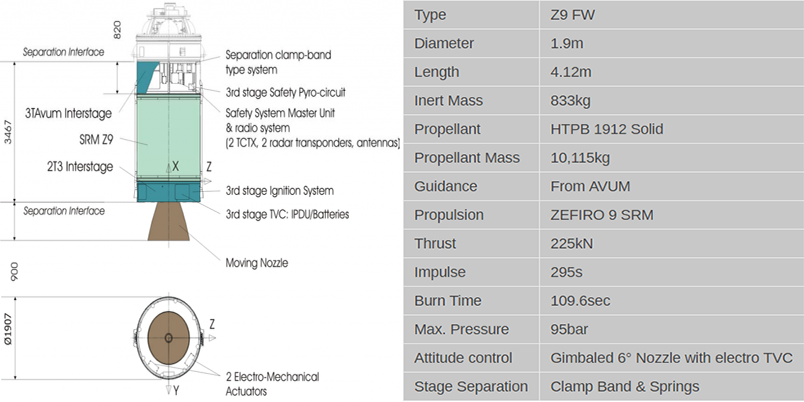
\includegraphics[width=1.0\textwidth]{Stage3.png}
    \caption{Vega Third Stage Configuration and Data}
    \label{fig:super}
\end{figure}

\begin{figure}[h]
    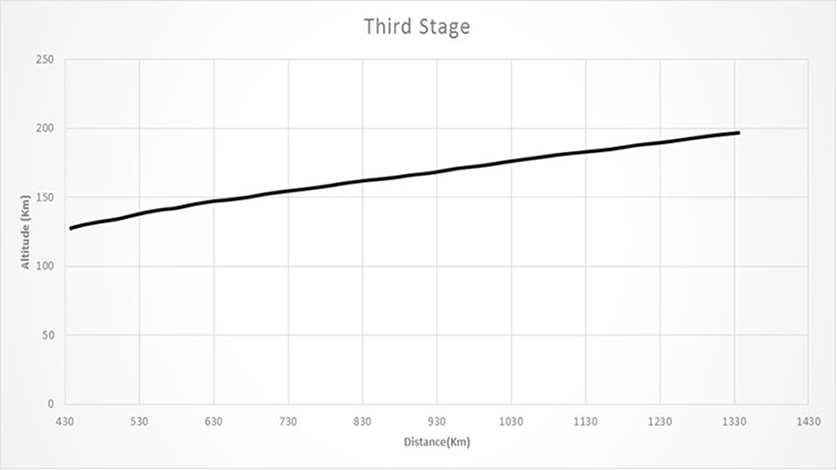
\includegraphics[width=0.567\textwidth]{Stage_3_Plot.jpg}
    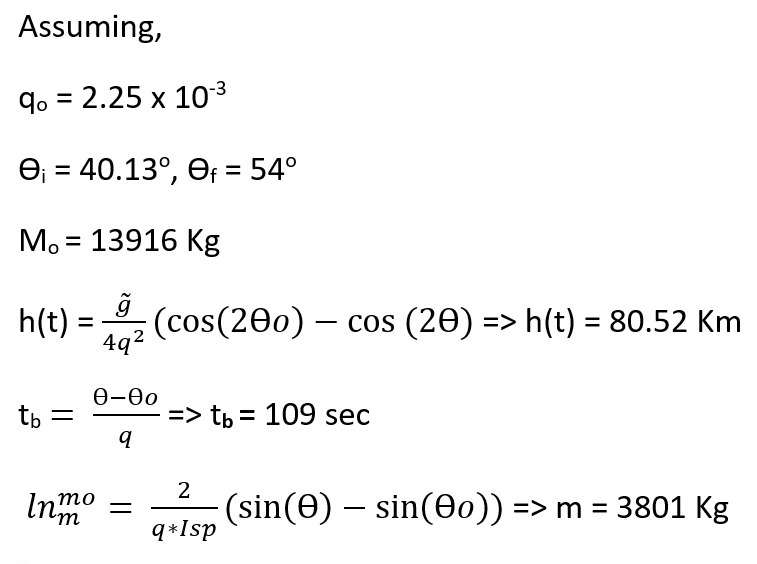
\includegraphics[width=0.433\textwidth]{Stage3_Cal.png}
    \caption{Stage 3 Trajectory Analysis}
    \label{fig:super}
\end{figure}
\clearpage
\subsection{Fourth/AVUM Stage}

The first burn of the Attitude and Vernier Upper Module (AVUM) multifunctional stage of the Vega Launch Vehicle burns for 593.35 seconds giving it an altitude of 428 Kilometers and velocity of 7302 m/s. 
	
\begin{figure}[h]
    \centering
    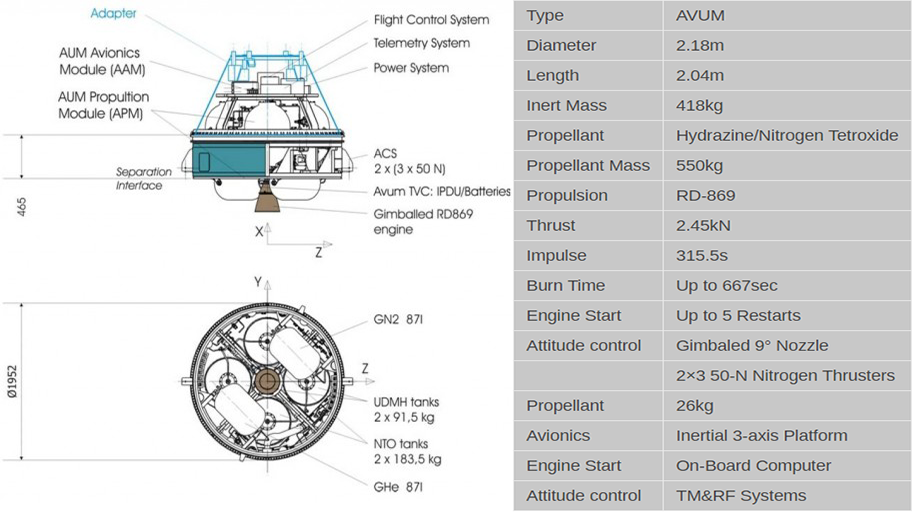
\includegraphics[width=0.82\textwidth]{Stage4.png}
    \caption{Vega Fourth/AVUM Stage Configuration and Data}
    \label{fig:pca}
\end{figure}
\begin{figure}[h]
    \centering
    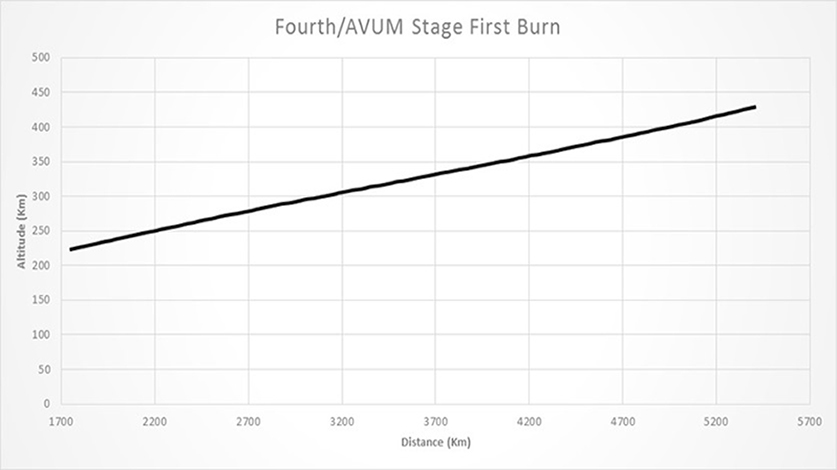
\includegraphics[width=0.82\textwidth]{Stage_4_Plot.jpg}
    \caption{Vega Fourth/AVUM Stage Configuration and Data}
    \label{fig:pca}
\end{figure}
\clearpage
\subsection{AVUM Second Burn and Final Separation}
After the first AVUM burn the vehicle coast for 85 minutes in an elliptical orbit. Again a second burn of 4th stage starts and and burns for 92 seconds giving the 1,906-kilogram LISA Pathfinder spacecraft a final orbit with apogee at 1,540 kilometers, and perigee at 207 kilometers, and an inclination of 5.96 degrees.

\begin{figure}[h]
    \centering
    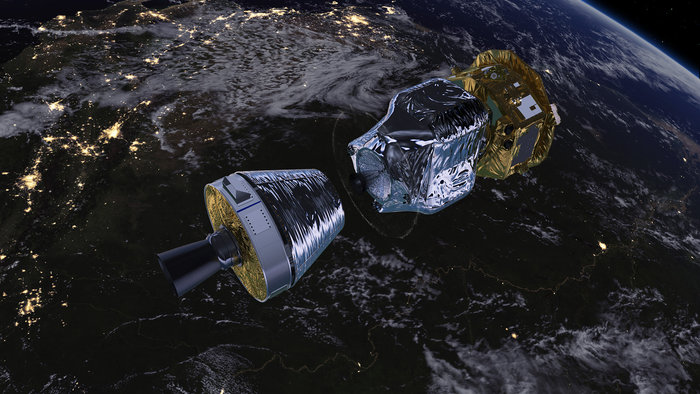
\includegraphics[width=0.82\textwidth]{Separation.jpg}
    \caption{LISA deploys from AVUM Fourth Stage of Rocket}
    \label{fig:pca}
\end{figure}
\clearpage

\chapterimage{Orbital.jpg}
\chapter{Orbital Manoeuvres}
\section{ARMs (Apogee Raising Manoeuvres)}\index{Related topics}
To travel to Sun-Earth L1 Point, LISA Pathfinder must raise its apogee to be near the 1.5-million-km point and to do so the spacecraft will perform a sequence of 'Apogee Raising Manoeuvres (ARMs) providing a velocity increment of more than 3000 m/sec  
\begin{figure}[h]
	\centering
    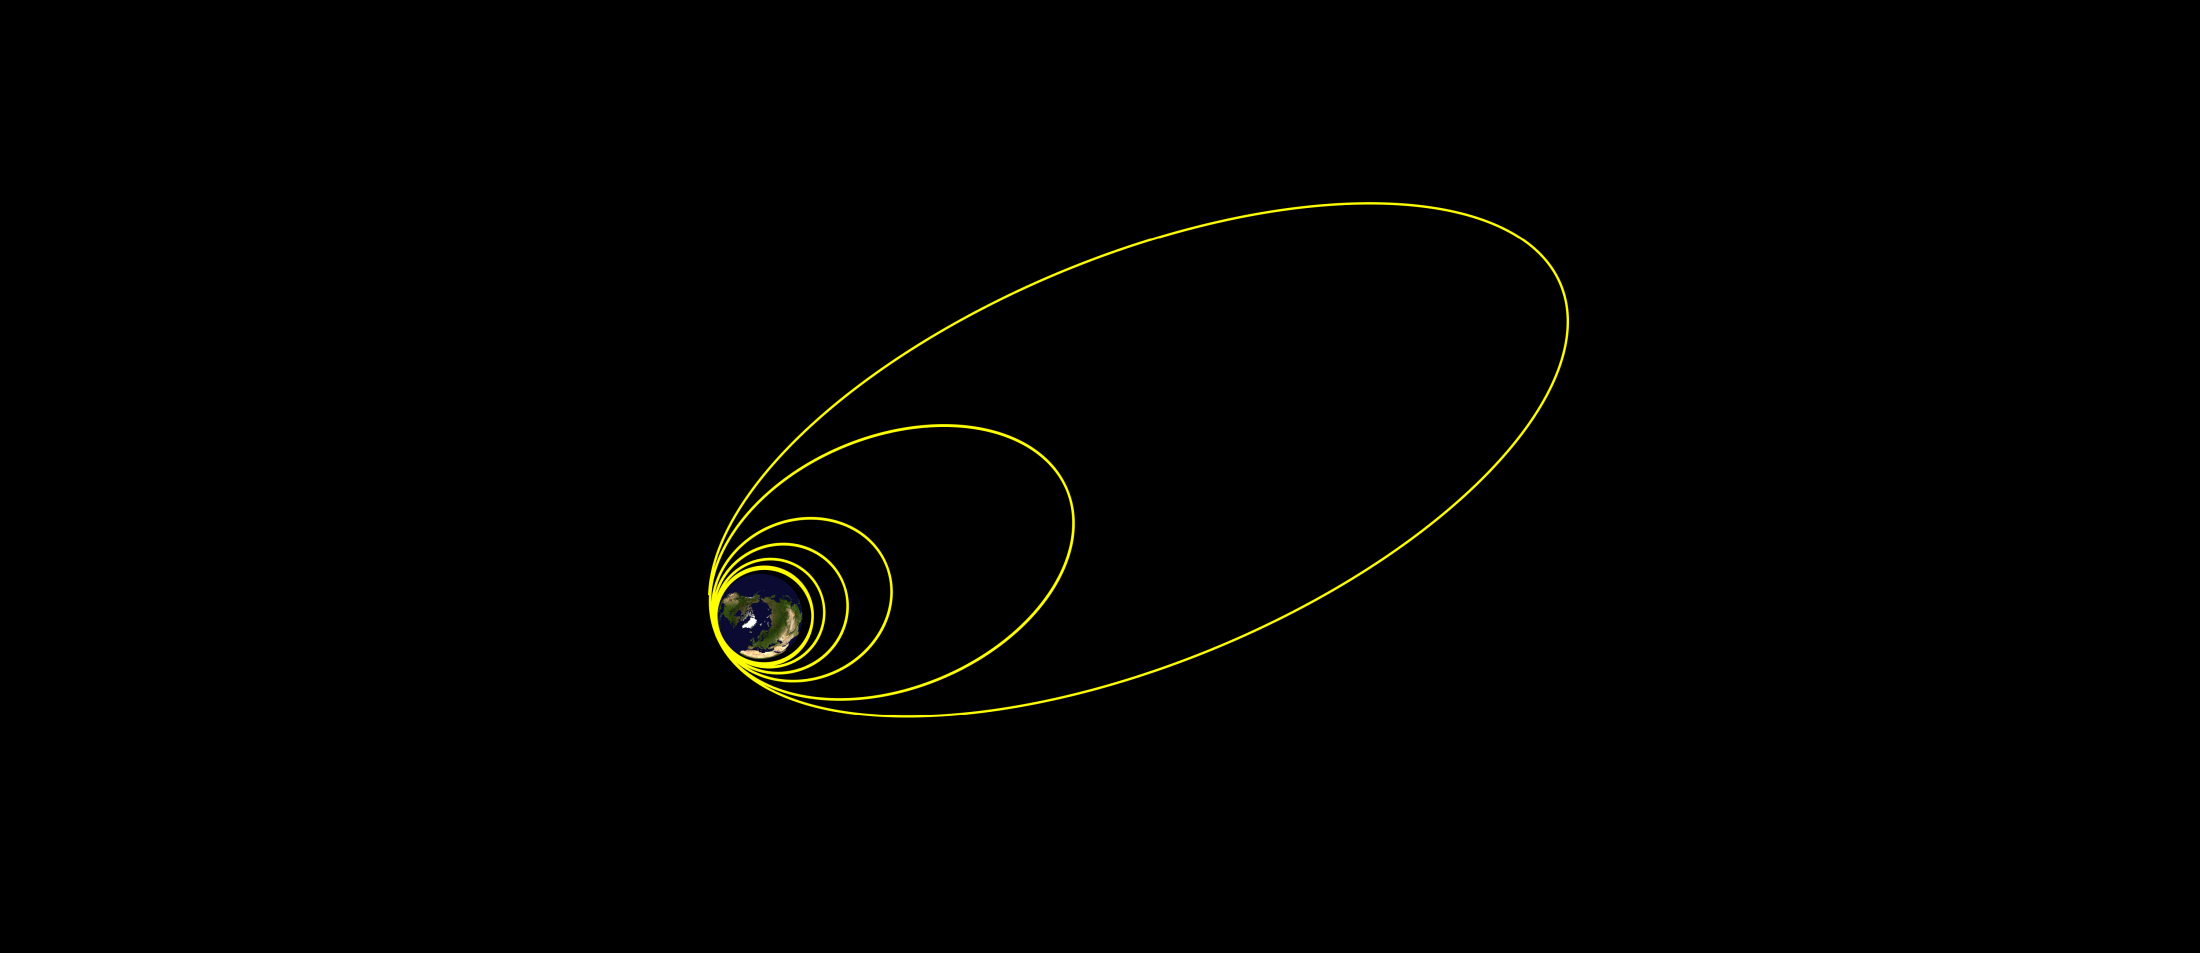
\includegraphics[width=1.0\textwidth]{APMs.png}
    \caption{All 6 ARMs of LISA}
\end{figure}

Before the Manoeuvres LPF was in an elliptical orbit with Perigee = 207 Km and Apogee = 1540 Km with an inclination of but 6.5 Degrees and total mass of 1910 Kg (including both fuel and instrumentation).
\clearpage

\subsection{ARM 1}\index{Related topics}

At the end of First Apogee Raising Manoeuvre:
\begin{description}
\item[New Perigee :] 207 Km
\item[New Apogee :] 1567 Km
\item[Delta Velocity :] 6.28 M/s
\item[Pre Burn Mass :] 1910 Kg
\item[Post Burn Mass :] 1905.63 Kg
\item[Required Mass :] 4.37 Kg
\end{description}

\begin{figure}[h]
    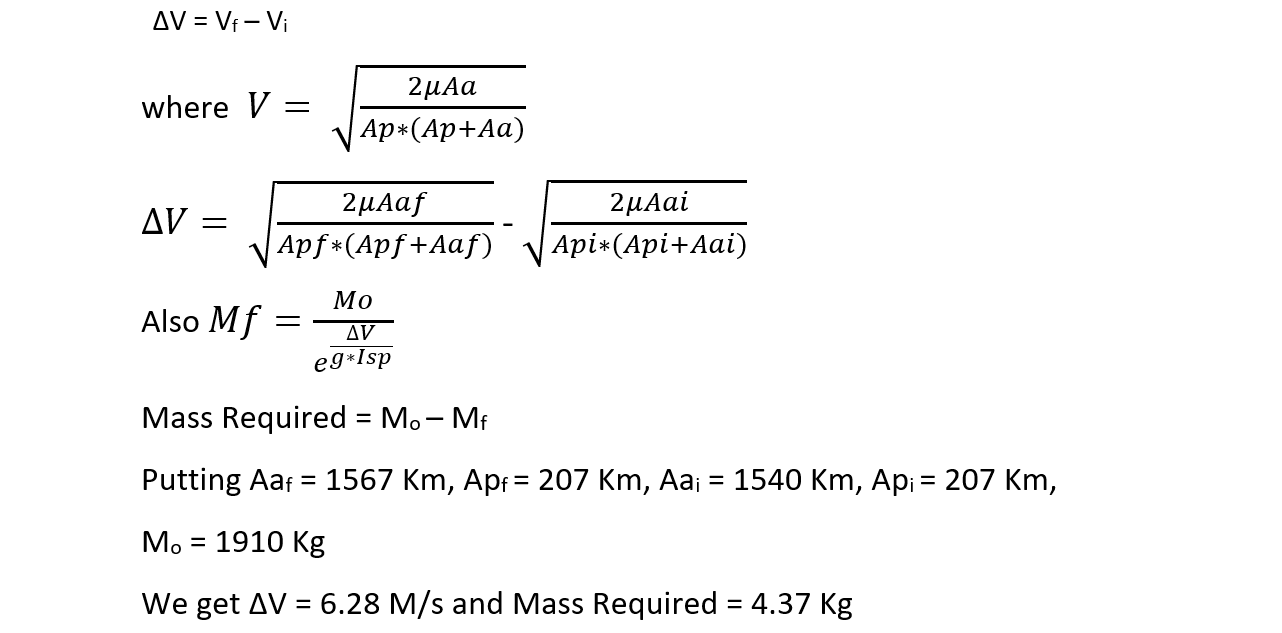
\includegraphics[width=0.8\textwidth]{ARM1.png}
\end{figure}

\subsection{ARM 2}\index{Related topics}

At the end of Second Apogee Raising Manoeuvre:
\begin{description}
\item[New Perigee :] 288 Km
\item[New Apogee :] 3392 Km
\item[Delta Velocity :] 295.23 M/s
\item[Pre Burn Mass :] 1905 Kg
\item[Post Burn Mass :] 1711.44 Kg
\item[Required Mass :] 194.19 Kg
\end{description}

\begin{figure}[h]
    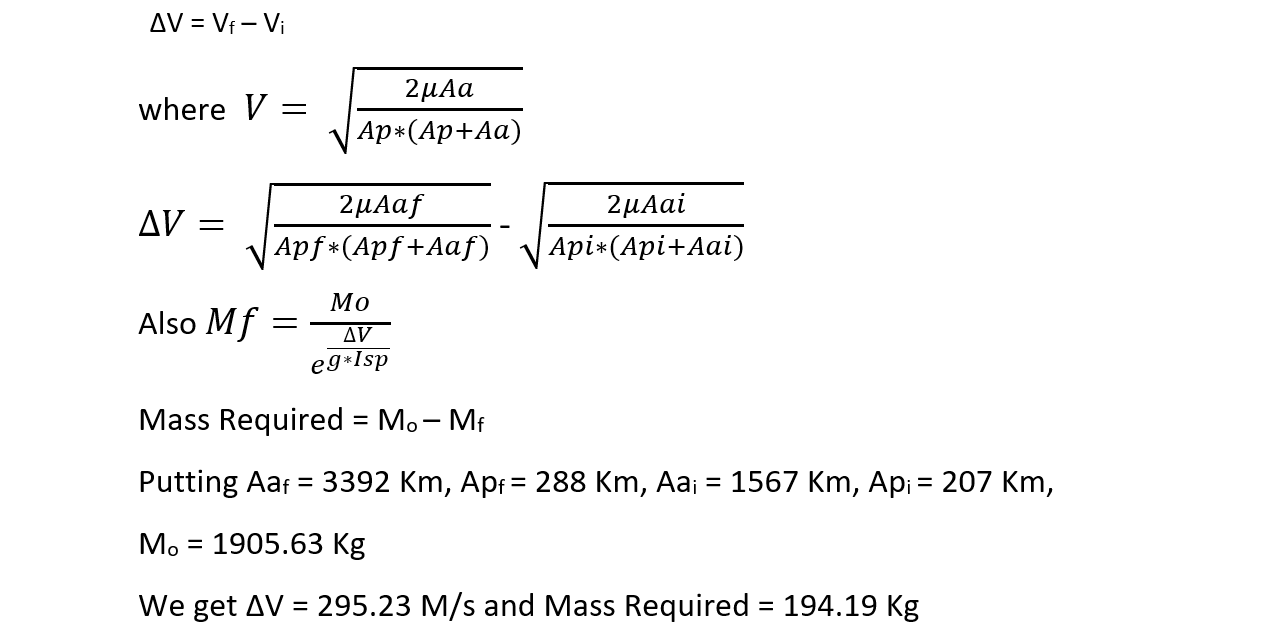
\includegraphics[width=0.8\textwidth]{ARM2.png}
\end{figure}
\clearpage
\subsection{ARM 3}\index{Related topics}

At the end of Third Apogee Raising Manoeuvre:
\begin{description}
\item[New Perigee :] 440 Km
\item[New Apogee :] 7091 Km
\item[Delta Velocity :] 379.36 M/s
\item[Pre Burn Mass :] 1711.44 Kg
\item[Post Burn Mass :] 1490.67 Kg
\item[Required Mass :] 220.77 Kg
\end{description}

\begin{figure}[h]
    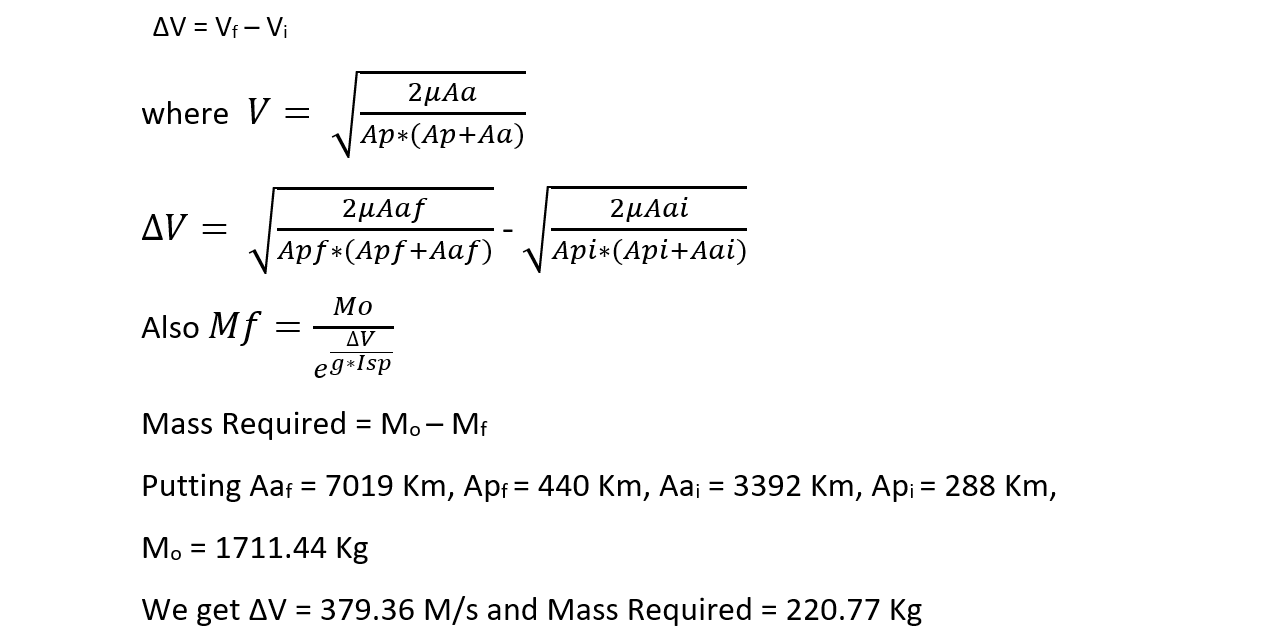
\includegraphics[width=0.8\textwidth]{ARM3.png}
\end{figure}

\subsection{ARM 4}\index{Related topics}

At the end of Fourth Apogee Raising Manoeuvre:
\begin{description}
\item[New Perigee :] 557 Km
\item[New Apogee :] 14137 Km
\item[Delta Velocity :] 458.06 M/s
\item[Pre Burn Mass :] 1490.67 Kg
\item[Post Burn Mass :] 1261.70 Kg
\item[Required Mass :] 228.97 Kg
\end{description}

\begin{figure}[h]
    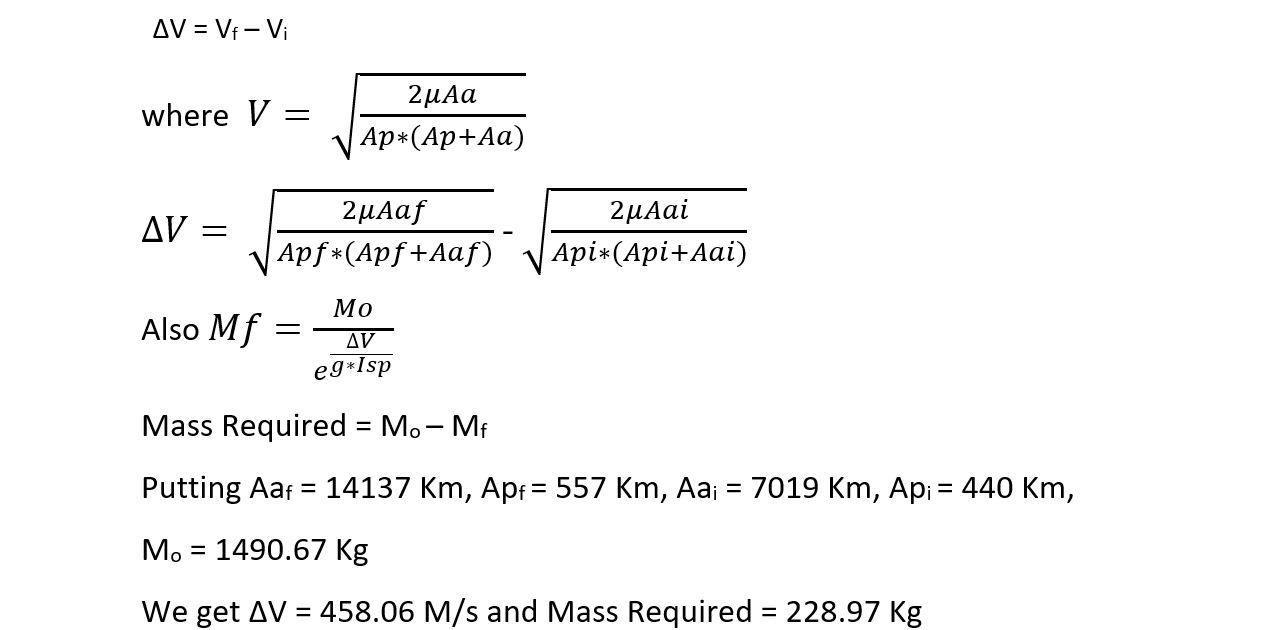
\includegraphics[width=0.8\textwidth]{ARM4.png}
\end{figure}
\clearpage

\subsection{ARM 5}\index{Related topics}

At the end of Fifth Apogee Raising Manoeuvre:
\begin{description}
\item[New Perigee :] 733 Km
\item[New Apogee :] 43641 Km
\item[Delta Velocity :] 638.43 M/s
\item[Pre Burn Mass :] 1261.70 Kg
\item[Post Burn Mass :] 1000.00 Kg
\item[Required Mass :] 261.70 Kg
\end{description}

\begin{figure}[h]
    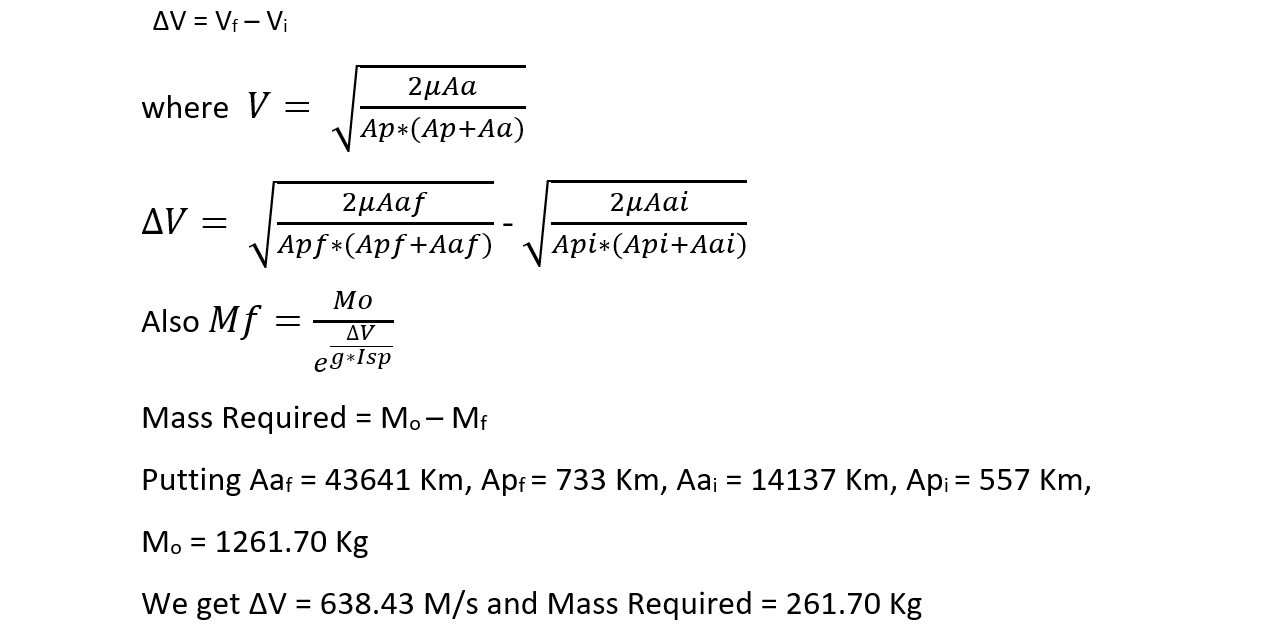
\includegraphics[width=0.8\textwidth]{ARM5.png}
\end{figure}

\subsection{ARM 6}\index{Related topics}

At the end of Sixth Apogee Raising Manoeuvre:
\begin{description}
\item[New Perigee :] 748 Km
\item[New Apogee :] 124805 Km
\item[Delta Velocity :] 393.62 M/s
\item[Pre Burn Mass :] 1000.00 Kg
\item[Post Burn Mass :] 866.52 Kg
\item[Required Mass :] 133.48 Kg
\end{description}

\begin{figure}[h]
    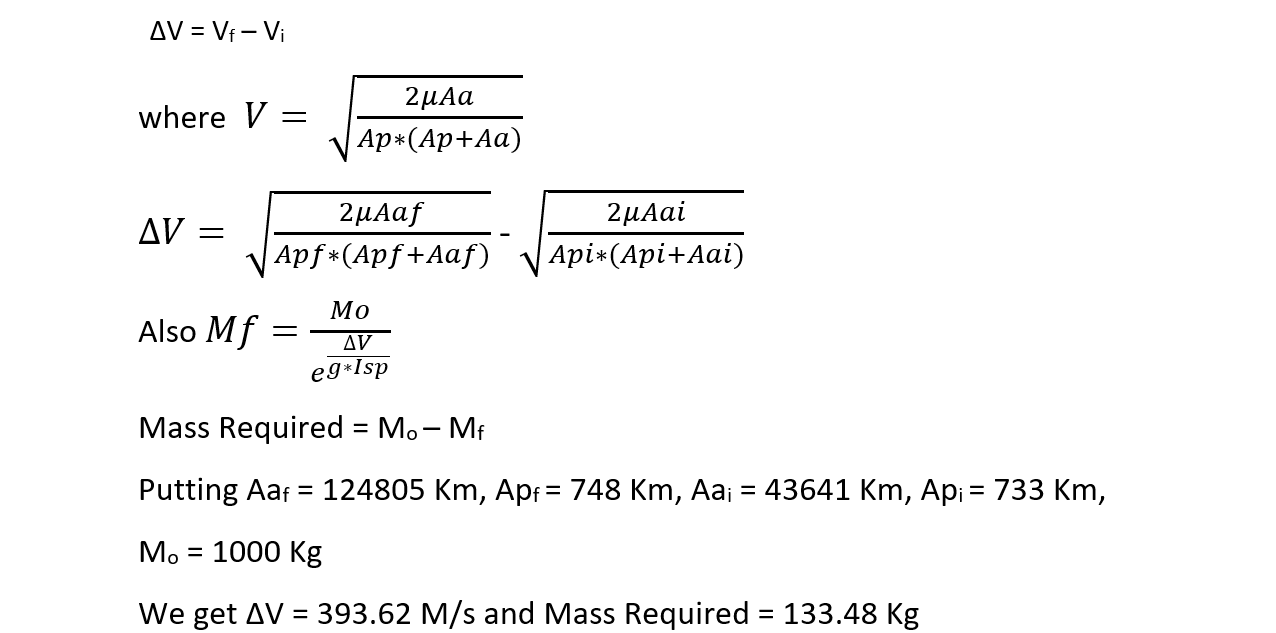
\includegraphics[width=0.8\textwidth]{ARM6.png}
\end{figure}
\clearpage
\chapterimage{FinalOrbit.png}
\chapter{Final Orbit}
\section{Operational Orbit}\index{Related topics}
The location of L1 is the solution to the following equation, balancing gravitation and the centrifugal force:

\begin{figure}[h]
	\centering
    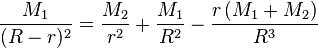
\includegraphics[width=0.35\textwidth]{Formula1.png}
\end{figure}

where r is the distance of the L1 point from the smaller object, R is the distance between the two main objects, and M1 and M2 are the masses of the large and small object, respectively. (The quantity in parentheses on the right is the distance of L1 from the center of mass.) Solving this for r involves solving a quintic function, but if the mass of the smaller object (M2) is much smaller than the mass of the larger object (M1) then L1 and L2 are at approximately equal distances r from the smaller object, equal to the radius of the Hill sphere, given by:

\begin{figure}[h]
	\centering
    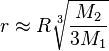
\includegraphics[width=0.12\textwidth]{Formula2.png}
\end{figure}
This distance can be described as being such that the orbital period, corresponding to a circular orbit with this distance as radius around M2 in the absence of M1, is that of M2 around M1, divided by sqrt{3}= 1.73:

\begin{figure}[h]
	\centering
    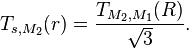
\includegraphics[width=0.23\textwidth]{Formula3.png}
\end{figure}
\clearpage

The operational orbit for LISA Pathfinder is a 500000 km x 800000 km Lissajous orbit around L1. This orbit has been chosen because it is an intrinsically 'quiet' place in space, far away from massive bodies, which induce tidal forces on the spacecraft; has constant illumination from the Sun; and has a quasi-constant distance from Earth for communication. This orbit fulfills the stringent requirements of LISA Pathfinder concerning thermal and gravitational stability.
This Lissajous orbit, with period of 180 days, is unstable and periodic station-keeping manoeuvres will be required - amounting to about 1.8 ms-1 per year - which will be performed using the cold gas thrusters of the spacecraft's micro-propulsion system.
\begin{figure}[h]
	\centering
    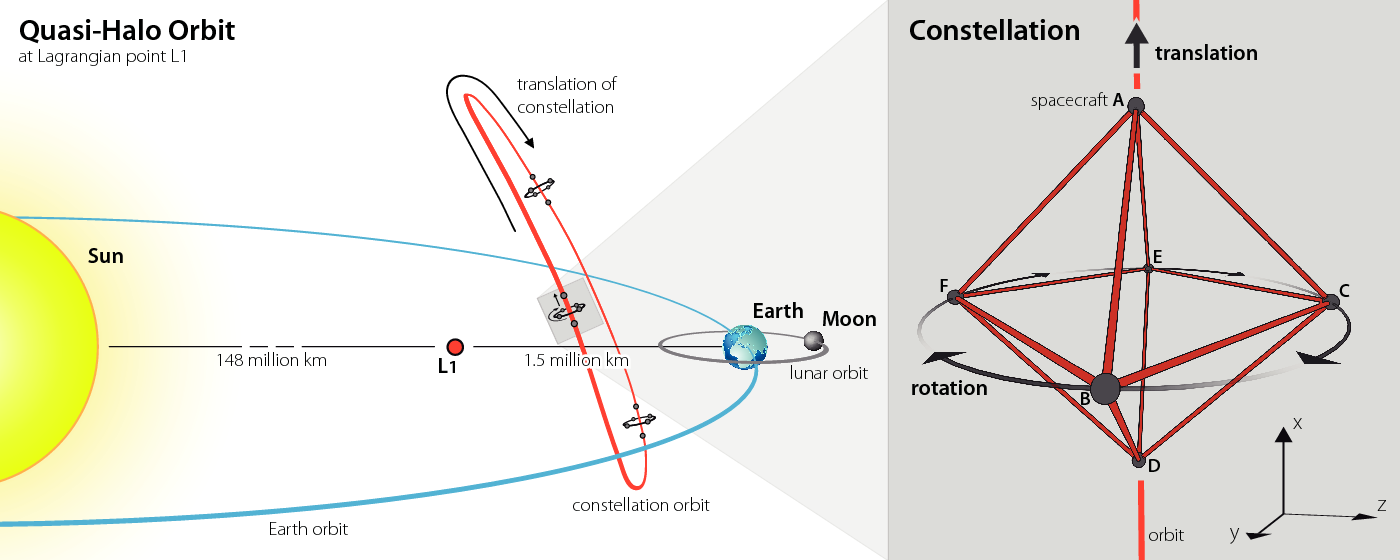
\includegraphics[width=1.0\textwidth]{L1_Orbit.png}
    \caption{Potato Chip type Orbit around Sun-Earth L1 point}
\end{figure}
\linebreak
For video Animation of LPF Orbit Visit:
\begin{description}    	  	  \item[]\url{http://www.esa.int/spaceinvideos/Videos/2015/10/LISA_Pathfinder_s_journey_to_L1}
\end{description}
\end{document}
